% 小时物理百科编辑器简介

\pentry{LaTeX 结构简介\upref{latxIn}}

\subsection{文件与目录}

小时物理百科使用统一的 \href{https://github.com/MacroUniverse/PhysWiki}{LaTeX 模板}, 主文件是根目录下的 \verb|main.tex|, 每个\textbf{词条}(即 \verb|\section|)占一个文件, 保存在 \verb|contents| 子目录中 (如 \verb|contents/Sample.tex|), 我们把它们叫做\textbf{词条文件}, 在编译 pdf 时词条文件会被插入 \verb|main.tex|.

在线编辑器新建的文件不是主文件, 而是被插入主文件的词条文件. 从编辑器打开文件时, 除第一项 \verb|main.tex| 外的所有文件也都是词条文件. 以下是一个词条文件示例(文件名 \verb|gougu.tex|)

\begin{lstlisting}
% 勾股定理

令 $a$, $b$ 和 $c$ 分别为直角三角形的两条直角边和斜边, 有
\begin{equation}
a^2 + b^2 = c^2
\end{equation}
\end{lstlisting}
保存(ctrl+s)后, 编辑器会自动给出网页预览, 如\autoref{latxIn_fig1}
\begin{figure}[ht]
\centering
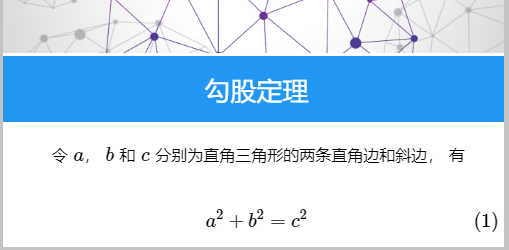
\includegraphics[width=11cm]{./figures/editIn_1.png}
\caption{在线编辑器预览} \label{editIn_fig1}
\end{figure}

注意词条文件中并不需要 \verb|\section{勾股定理}|, 因为它会被直接插入主文件. 但为了查看方便, 我们规定每个词条第一行必须注释词条标题.

完成编写词条后, 我们需要在主文件 \verb|main.tex| 中插入该词条. 在编辑器中打开主文件, 在适当的章节中插入 \verb|\entry{勾股定理}{gougu}| 即可\footnote{\verb|\entry| 是模板定义的, 相当于 \verb|\section{勾股定理}\label{gougu}\input{./contents/gougu}|}. 保存后, 我们就可以在\href{http://wuli.wiki/changed}{百科目录}中看到这个词条了\footnote{如果你在使用个人笔记功能, 则会显示到个人笔记目录中}, 如果编译 pdf 也可以在 pdf 的目录中看到.

注意新建和修改的词条页面(html)会暂存在草稿区(\href{http://wuli.wiki/changed/}{wuli.wiki/changed/}), 只有有权限的用户发布后才会转移到正式目录 (\href{http://wuli.wiki/online/}{wuli.wiki/online/}).
